

\section{Data Management Organization Structure}
This section defines the organization structure for the period in which the DM System is developed and commissioned, up to the start of LSST Observatory operations.  
(\appref{sect:precon} gives historical  Pre-Construction Phase Organization).

The DM Project Manager and DM Project Scientist, who are known collectively as DM Management, lead the DM Subsystem.  The Project Manager has direct responsibility for coordination with the overall LSST Project Office, the LSST Change Control Board, the LSST Corporation, and LSST partner organizations on all budgetary, schedule, and resource matters.  The Project Scientist has primary scientific and technical responsibility in the DM and responsibility for ensuring that the scientific requirements of the LSST are supported, and is a member on the LSST Project Science Team (PST). 

As shown in \figref{fig:dmorg}, the organization now features lead institutions, each with responsibility for major element of the DM System (Level 2 Work Breakdown Structure elements).  For example, during Final Design, the Process Control and Archive Site Manager and Team at NCSA will be conducting prototyping activities in computing, data communications, and data storage to select and verify the ability of System technologies to support the LSST requirements.  They will also be involved in creating a supporting infrastructure for the DM Systems.  During Construction before the LSST first light time frame, these resources will be focused on implementation of the selected technologies.  In order to ensure that team functions as one integrated project, the institutions coordinate support by other lead institution team members directly through this organizational structure, as well as via a number of cross-organizational bodies (described later in this document). 
Also, due to the span of the organization, the DM Project Manager may be supported by one of the lead institution Project Managers as a Deputy Project Manager in these phases.

\begin{figure}[htbp]
\begin{center}
 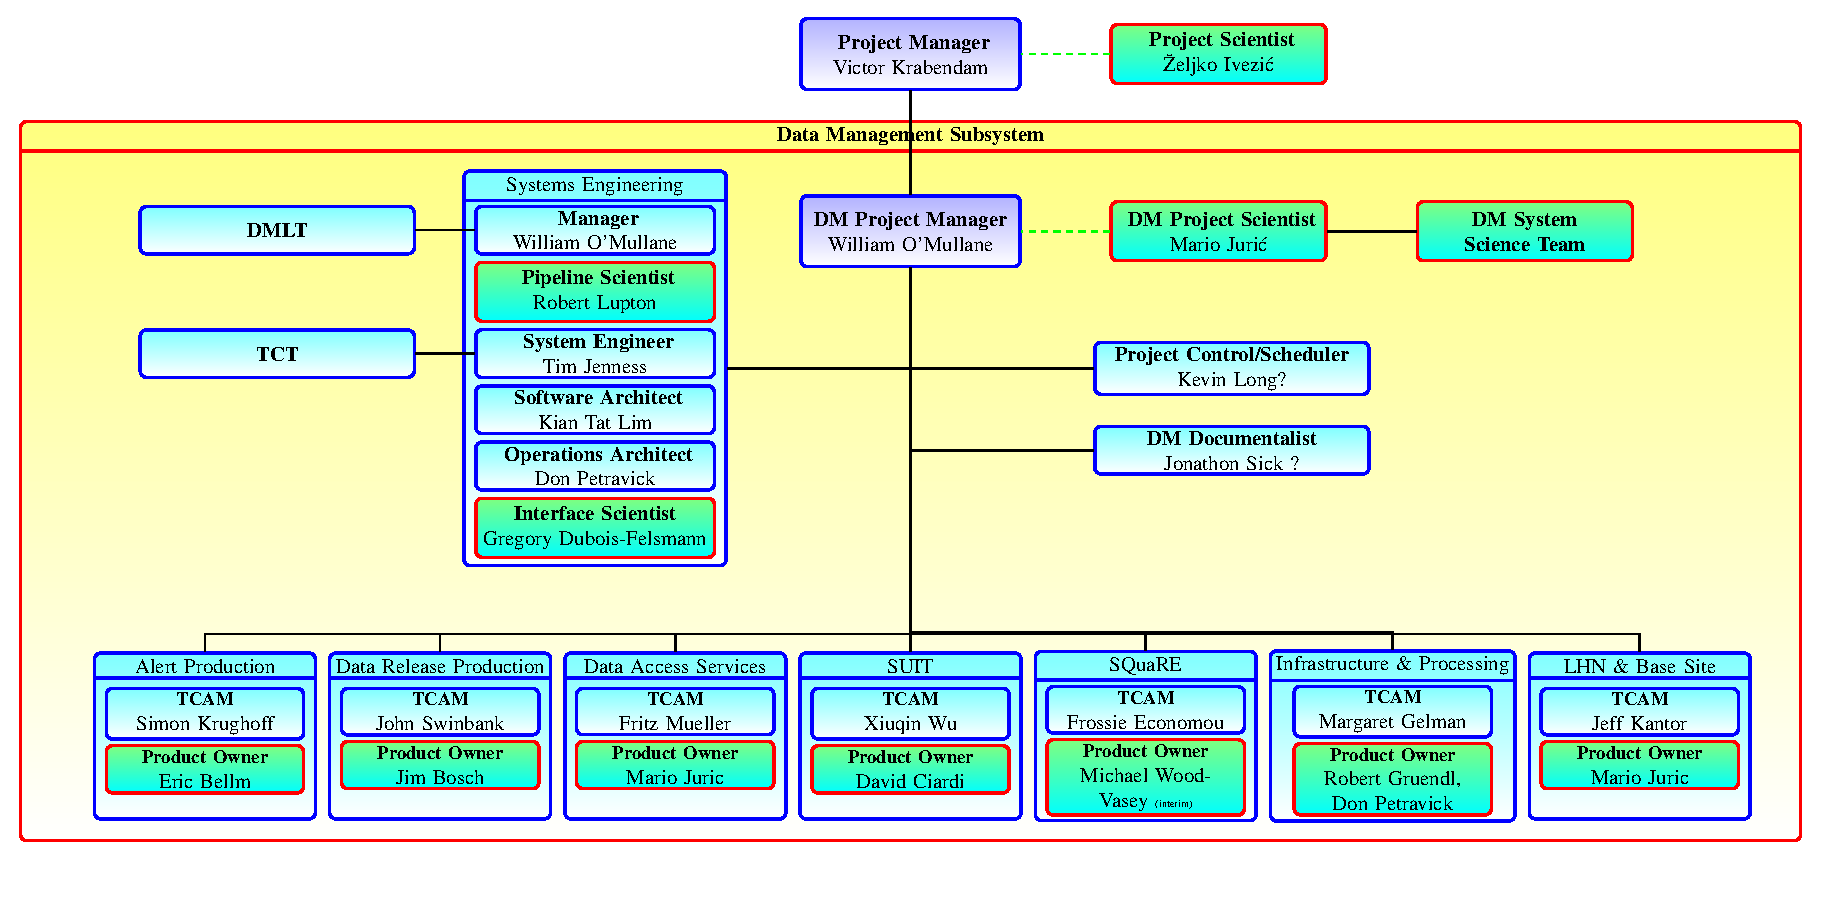
\includegraphics[width=\textwidth]{images/DmOrg}
\caption{DM organisation with Scientists in Green. \label{fig:dmorg}}
\end{center}
\end{figure}

\subsection {Document Management}
DM documents will follow the System Engineering Guidelines of LSST. PDF versions of released documents shall be put in Docushare. 

The Document Tree for DM is shown in \figref{fig:doctree}, it is not exhaustive but gives a high level orientation for the main documents in DM and how they relate to each other.

\begin{figure}
\begin{center}
 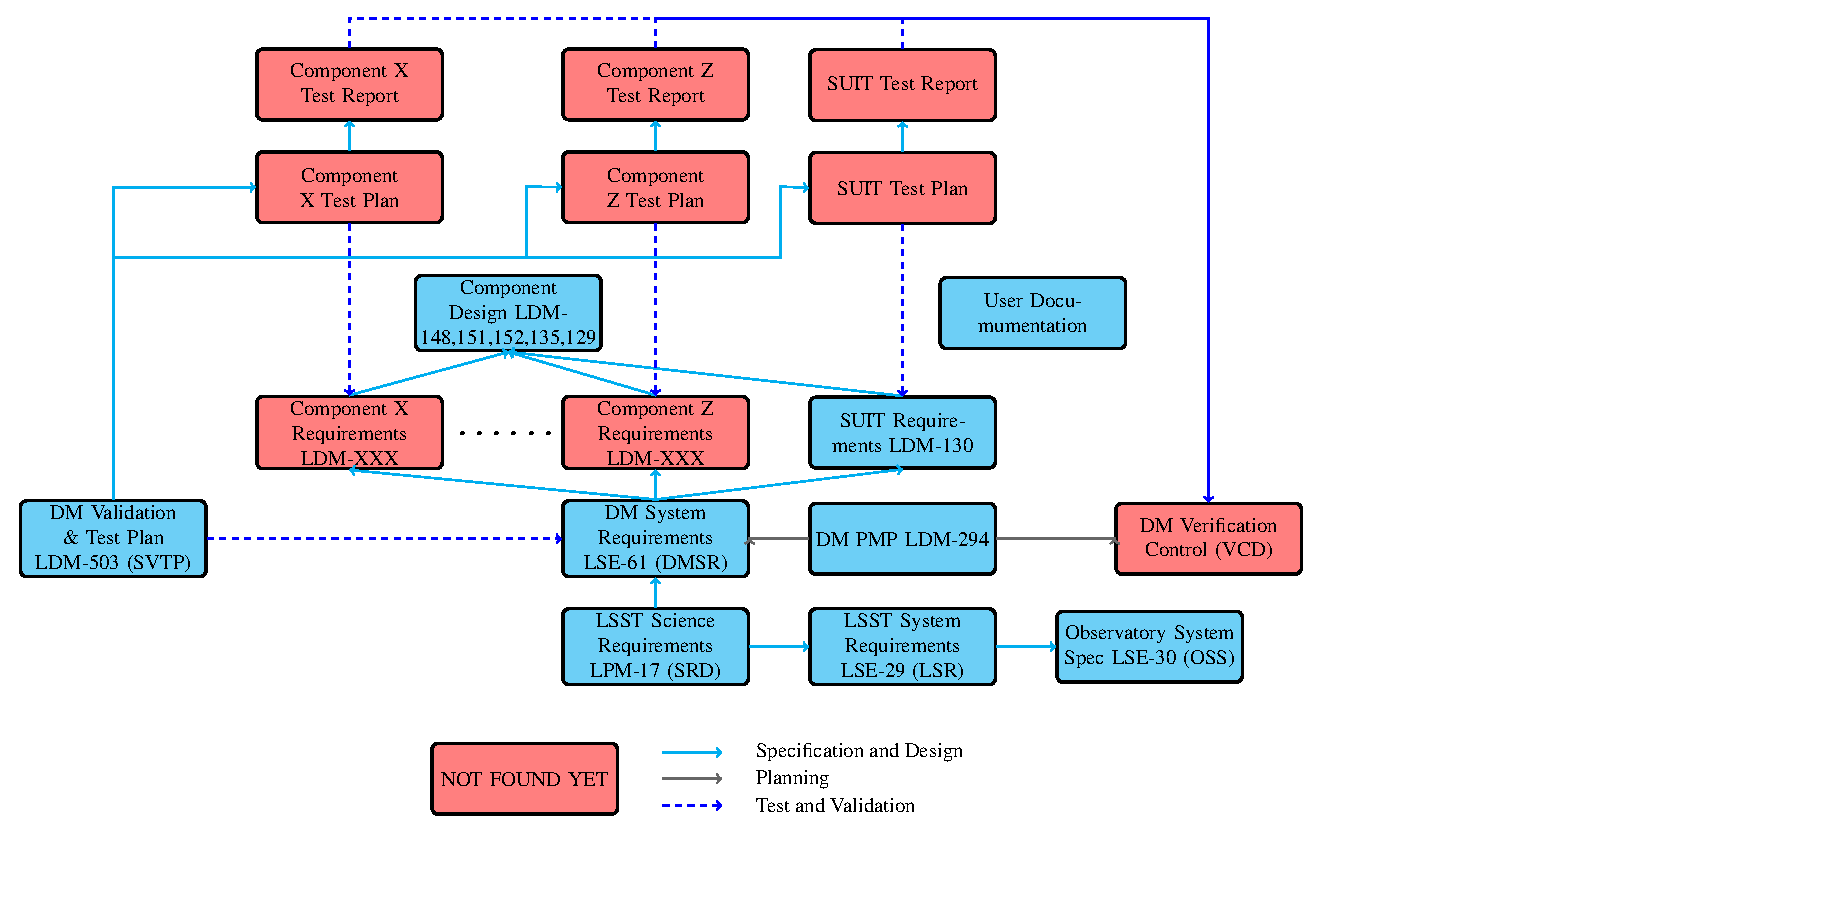
\includegraphics[width=0.8\textwidth]{images/DocTree}
\caption{Outline of the documentation tree for DM relating the high level documents to each other. \label{fig:doctree}}
\end{center}
\end{figure}

\subsection {Configuration Control }
\subsection {Risk Management }
\subsection {Product Assurance  }

\section{Roles in Data Management}

There are many roles listed in \figref{fig:dmorg}, this section enumerates responsibilities going with those roles. 


\subsection{DM Project Manager \label{role:dmpm}}

The DM Project Manager is responsible for the efficient coordination of all LSST activities and responsibilities assigned to the Data Management Subsystem. The DM Project Manager has the responsibility of establishing the organization, resources, and work assignments to provide DM solutions.  The DM Project Manager, serves as the DM representative in the LSST Project Office and in that role is responsible for presenting DM initiative status and submitting new DM initiatives for approval consideration. Ultimately, the DM Project Manager, in conjunction with his / her peer Project Managers (Telescope, Camera), is responsible for delivering an integrated LSST system. The DM Project Manager reports to the LSST Project Manager. Specific responsibilities include:

\begin{itemize}
\item Manage the overall DM System
\item Define scope and funding for DM System 
\item Develop and implement the DM project management and control process, including earned value management
\item Approve the DM Work Breakdown Structure (WBS), budgets and resource estimates
\item Approve or execute as appropriate all DM outsourcing contracts 
\item Convene and/or participate in all DM reviews
\item Co-Chair the DM Leadership Team
\end{itemize}

\subsection{DM Project Scientist \label{role:dmps} }
The DM Project Scientist has ultimate responsibility for ensuring DM initiatives provide solutions that meet the overall LSST scientific and technical requirements.  The DM Project Scientist must ensure correct specification of DM Scientific Requirements and proper translation of those requirements into derived information technology requirements and ultimately, into implemented solutions.  The DM Project Scientist must ensure that the DM subsystem is properly scoped and integrated within the overall LSST system.  The DM Project Scientist is also a member of the LSST Project Science Team (PST) and reports to the LSST Director. Specific responsibilities include:

\begin{itemize}
\item Responsible for the science deliverables of the DM System
\item Set requirements for the DM that:
\begin{itemize}
\item Ensure that the design and operational flow of the data products meet the needs of the science community
\item Ensure that the quality requirements of the data products will be / are being met by the DMS, with a particular emphasis on choice of appropriate application algorithms
\end{itemize}
\item Set requirements for and assess/validate results of Data Challenges and other precursor experiments
\item Set requirements and assess/validate results for Data Releases
\item Convene and/or participate in all DM reviews
\item Co-Chair the DM Leadership Team and Science/Architecture Team
\end{itemize}

\subsection{ Project Controller/Scheduler \label{pcon}}
Keep AGILE plan in sync with the overall LSST planning (primavera), track milestones from TCAMS \secref{role:tcam}. 
Help TCAMS with building the plan from the milestones tracking dependencies and keeping it up to date. 

Help set up sprint - points available (start/end day, account for holidays etc.) 
Bug team in general about story status in sprints and their tracking status (points spent).

Create reports and gannt charts for the DM Project Manager as needed \secref{role:dmpm}
\subsection{Technical Control/Account Manager (TCAM) \label{role:tcam} }
Accountable for planning and execution in their area. Reporting to the DM Project Manager \secref{role:dmpm}. In AGILE could also be seen as the SCRUM Master for the local team.

\subsection{ Product Owner \label{role:prodo }}
The product owner, aka. the X scientist (where X is the product e.g. Alerts Production), is responsible for the product quality and acceptance. 
The product owner should sign off on the requirements to be fulfilled in every delivery and therefore also on any descopes or enhancements. 
The Product owner should define tests which can be run to prove a delivery meets the requirements due for that product. 

\subsection{Pipeline Scientist \label{role:pipe }}
Several DM products come together to form the LSST pipeline. The Pipeline Scientist is the product owner for the overall pipeline. 
The Pipeline Scientist should :
\begin{itemize}
\item  Provide guidance and test criteria for the full pipeline including how QA is done on the products.  
\item Keep the big picture of where the codes are going in view. Predominantly the algorithms, but also the implementation and architecture (as part of the System Engineering Team \secref{sect:sysengt}).


\item Advise on how we should attack algorithmic problems,  
providing continuing advice to subsystem product owners as we try new things. 

\item Advise on calibration issues, provide understanding of the detectors from a DM point of view. 

\item Advise on the overall (scientific) performance of the system, and how we'll test it.  Thinking about all the small things that we have to get right to make the overall system good.



\end{itemize}


\subsection{System Engineer \label{role:sysengineer }}
With the system engineering team \secref{sect:sysengt} 
 the System engineer 
 owns the DM entries in the risk register and is generally in charge or the {\em process} of building DM products. 

The System engineer  
is responsible for the requirements work:
\begin{itemize}
\item E.g., updating the DMSR, OSS, LSR (including traceability)
\item Ensure we’re appropriately modelling and recording information about the system (e.g.,
    drawings, design documents, etc.)
\item Overseeing work on ICDs, lower level requirements documents, etc.
\item Ensuring we have a solid verification plans/standards across the board in DM
\end{itemize}

The System Engineer is responsible for the process to define \& maintain DM interfaces
\begin{itemize}
\item Defining standards for and ensuring internal interfaces are identified and worked out
\item Direct Interface Scientist's work on external ICDs
\end{itemize}

The System Engineer shall Chair the DM Technical Control Team \secref{sect:tct}
\begin{itemize}
\item Organise TCT processes so our change control process runs smoothly
\item Shepherd RFCs through change control
\item Monitor + Flag RFCs requiring TCT attention
\item Call up meetings, make sure decisions are made, and recorded
\end{itemize}

The System Engineer represents DM on the CCB
\begin{itemize}
\item Shepherd DM’s CRs through the CCB
\item Serve as the Point of Contact for DM on the CCB
\end{itemize}

\subsection{Requirements Engineer \label{role:reqeng }}
With the system engineering team \secref{sect:sysengt} and in close coordination with the software architect (\secref{role:softarc} and the system engineer \secref{role:sysengineer} look after the baseline requirements for DM.. 


\subsection{Software Architect \label{role:softarc }}
{\bf to be written}
The software architect looks after the software we are building. How does it all fit together are their techniques/technologies we should be using. How can we minimise dependencies. 

With the \secref{role:sysengineer} the Software architect should also agree how to track requirements to code and verify requirements are i.e. are hooks required in the code ?
\subsection{Operations Architect \label{role:sysarc }}
The DM System Architect is responsible for ensuring that all elements of the DM systems, including operations teams, infrastructure, middle ware, applications, and interfaces, i
come together to form an operable system. 
Specific responsibilities include:
\begin{itemize}
\item Setting up and coordinating  Operations Rehearsals
\item Ensuring Readiness of procedures and personnel for Operations
\item Set standards for operations e..g procedure handling and operator logging
\item Participate in stakeholder and end user coordination and approval processes and reviews
\item Member of the LSST System Engineering Team
\end{itemize}


%\subsection{ \label{role: }}

\section{Data Management Groups/Bodies}
Since the DM team is distributed in terms of geography and responsibility across the LSST partner and lead institutions, mechanisms are needed to ensure that the project remains on track at all times.  There are three primary coordinating bodies to ensure the management, technical, and quality integrity of the DM project.  All DM institutions have membership on these bodies, and all meet at least once per month during construction and commissioning.

\subsection{DM Science Performance/Validation Team?}
Run by DM PS .. tell us if we meet the science goals - investigate problems, analyse commissioning data. 
\subsection{DM System Engineering Team \label{sect:sysengt}}
Look after requirements traceability, interfaces, ..

\subsection{DM Leadership Team}

The DM Leadership Team (DMLT) purpose is to establish scope of work and resource allocation across DM and ensure overall project management integrity across DM.
The following mandate established the DMLT:

\begin{itemize}
\item Charter/purpose
	\begin{itemize}
	\item Maintain scope of work and keep within resource allocation across DM
	\item Ensure overall project management integrity across DM
	\item Ensure Earned Value management requirements are met
	\end{itemize}
\item Membership
	\begin{itemize}
	\item Co-Chaired by the DM Project Manager  and  DM Project Scientist
	\item Core members are Lead Institution Technical/Control Account Managers (T/CAMs or CAMs)
	\end{itemize}
\item Responsibilities
	\begin{itemize}
	\item Prepares all budgets, schedules, plans
	\item Meets every week to track progress, address issues/risks, adjust work assignments and schedules, and disseminate/discuss general PM communications
	\item Creates and publishes monthly, quarterly, annual progress reports
	\item Meets at start of each software development phase with SAT to establish detailed scope/work plan
	\item Meets with SAT for change control (TCT)
	\end{itemize}
\end{itemize}

The DM Leadership Team and the System Engineering Group (\secref{sect:sysengt} work in synchrony. 
The DMLT makes sure the requirements and architecture/design are estimated and scheduled in accordance with LSST Project required budgets and schedules.



\subsection{Technical Control Team \label{sect:tct}}
The DM Technical Control Team has responsibility for issues similar to those of the LSST Configuration Control Board, but restricted to those contained within the DM subsystem. The TCT reviews and approves changes to all baselines in the LSST Data Management System, including proposed changes to the DM System Requirements' (DMSR), reference design, sizing model, i.e. any LDM-xxx baseline document.  The TCT makes sure these changes don't get into the baseline without proper change control.  Note that the TCT does not author the Technical Baseline and has no specific technical deliverable charter, but it does validate that the form and content of the Technical Baseline is consistent with LSST project standards such as the System Engineering Management Plan (SEMP).  Specific responsibilities for development of the Technical Baseline and evaluation of the content versus LSST and DM requirements are elsewhere in this document.
\begin{itemize}
\item Charter/purpose
	\begin{itemize}
	\item Ensure that the DM Technical Baseline (LDM-xxx) documents are baselined and once baselined only changed when necessary, according to LSST and DM configuration control processes
	\end{itemize}
\item Membership
	\begin{itemize}
	\item Chaired by the System Engineer
	\item Members include the DM System Architect, DM System Interfaces Scientist, DM SQuaRE Technical Manager and DM Project Manager
	\item For on-line virtual meetings, if a quorum is not reached within one week, the DM Project Manager will make a unilateral decision
	\end{itemize}
\item Responsibilities
	\begin{itemize}
	\item Determines when specification and deliverables are of sufficient maturity and quality to be baselined (placed under configuration controlled status) or released. The TCT reviews and approves proposed changes to baselined items.
	\item Reviews and approves/rejects proposed changes to baselined items
	\end{itemize}
\end{itemize}



